\documentclass[JohnsonMADraft2.tex]{subfiles}
\begin{document}
\doublespacing 
\subsection*{Defining Judicial Independence}%Why the fuck do we Care
Latent concepts are inherently difficult to measure.  They can refer to broad and abstract concepts like democracy, respect for human rights, judicial independence, or smaller concepts such as the ability to do math or reading comprehension, commonly used in educational testing, to the slightly absurd such as knowledge of Star Trek or Star Wars \citep{Jackman2008, Treier2008,Schnakenberg2014,Linzer2014}.  The first task in attempting to measure a latent concept is to find a common definition.  

There has been many definitions put forth for judicial independence.  ``Judicial independence can and should be defined as among other things the institutional arrangements designed to protect the judiciary from the executive and the public at large,'' \citep[131]{Tiede2006}.  Tiede presents an abstract conceptualization that is difficult to operationalize.   \citet[108]{McNollgast2006} come up with a more narrow, but equally abstract characterization of  judicial independence ``as an outcome that emerges from strategic interactions among the judiciary, the legislature, and the executive.''  \citet[286]{Howard2004} define judicial independence as ``the extent to which a court may adjudicate free from institutional controls, incentives, and impediments imposed or intimidated by force, money, or extralegal, corrupt methods by individuals or institutions outside the judiciary, whether within or outside government.''  \citet[4]{Linzer2014} use a slightly different definition, stating that a judge is independent ``in so far as her decisions reflect her evaluation of the legal regard and in so far as those decisions are respected by government officials.''

\citet{Rios2006} present judicial independence as a principal-agent relationship.  ``A relationship between those who delegate, in contemporary democracies the politicians that populate the elected branches of government, and the delegates or the judges in this case,'' \citep[6
]{Rios2006}   While R\'{i}os-Figueroa's study was designed for a cross-national comparison, this definition is well suited for adaptation in the American context.  Rather than simply being the politicians in the elected branch of government, this includes delegation from the voters to the judges though direct elections.  \citet[17]{Rios2006} formalizes this association as follows: ``a relation between an actor ``A'' that delegates authority to an actor ``B'', where the latter is more or less independent of the former depending on how many controls A retains over B.''  In the American context this can be viewed as either the voters or the governor's control over retention of judges.  While voters and governors cannot directly control the decisions that a judge makes, they do exercise considerable power over the retention of judges.  

As noted above, one of the challenges in studying the latent variable of judicial independence is that researchers do not share a common conceptual definition of independence \citep{Linzer2014}.  There is some common ground to these definitions however.  Most definitions of judicial independence agree that an independent judge should be free to make her own decisions without regard to pubic opinion, or ruling party positions.  They also agree that independent judges should not be intimidated by the public or the government as a consequence of any particular ruling.\footnote{As \citet[4]{Rios2014} note, parties and governments put pressure on judges during proceedings by filing \textit{amicus curiae} briefs and other methods, however, these are perfectly legal within the system.}  How do judicial systems protect judges from these types of threats to their independence?  To answer this question we need to further deconstruct the definition of judicial independence. 

%Accountability vs. Independence
\subsection*{The Judicial Independence Continuum}
``Judicial independence is merely the other side of the coin from judicial accountability, \citep{Burbank2008}.  Many of the institutional rules that remove independence serve the opposite function of creating accountability for judges.  \citet{Hall2007} defines two premises of judicial accountability. The first is the simple idea that citizens have accountable control over judges through the ballot box, and the second is the ``willingness of challengers to enter the electoral arena and the propensity of the electorate not to give their full support to incumbents'' \citep[166]{Hall2007}.

Figure \ref{IndCon} illustrates how rather than being dichotomous or ordinal, independence and accountability can more properly be considered as a continuum.  The Judicial Independence Continuum is a single dimension continuum comprising total accountability on one side with a totally accountable judiciary on one side with a totally independent judiciary on the other.  As a judicial institution moves across he indicators described below in Section \ref{Indicators}, it changes position on the Independence Continuum. 

%Independence Continuum
\begin{figure}[tb]\centering\caption{Judicial Independence Continuum}\label{IndCon}
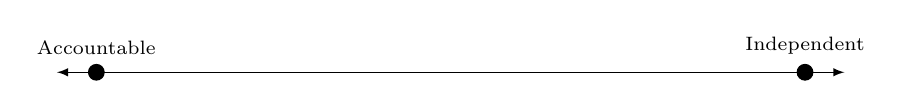
\begin{tikzpicture}
% a straight line segment
\draw[latex-latex] (-0.5,0) -- (9.5,0);
%% the labels
\node[fill=black,draw=black,circle,inner sep=2pt,label=above:{\scriptsize Independent}] at (9,0) {};
\node[fill=black,draw=black,circle,inner sep=2pt,label=above:{\scriptsize Accountable}] at (0,0) {};
\end{tikzpicture}
\end{figure}

Judicial independence takes two forms: \textit{de jure} and \textit{de facto} \citep{Feld2003,Rios2014, Rosenberg1991,Voeten2008}.  \textit{De facto} judicial independence reflects two concepts: first, a judge is independent when her decisions reflect her preferences, and second, even if a court is totally independent ``that lacking financial or physical means of coercion, courts depend on the assistance of other political authorities to enforce their decisions'' \citep[4]{Rios2014}. Can a judge with a set term of office reasonably expect to remain in office no matter which way they rule on a particular case? If the answer to that question is yes, the judge enjoys \textit{de facto} independence. 

\citet[3]{Rios2014} define \textit{de jure} judicial independence as ``formal rules designed to insulate judges from undue pressure, either from outside the judiciary or within.''  These are the institutional protections that allow a judge to be independent from the executive, public, legislature, or superior courts.  Examples of these protections include selection and retention methods, term lengths, and docket control.

Judicial independence itself is a latent concept, meaning that is cannot be measured directly \citep[203]{Treier2008}.  However, there exist indicators that allow us to measure both \textit{de jure} and \textit{de facto} judicial independence.  As \citet[5]{Rios2014} note, the indicators used to measure \textit{de jure} independence are easily observable, however, measuring the latent variable of independence is what is far more challenging.  Judicial independence is not a new concept, it has been examined for many years.  Owing to the latency of the concept, it has proven routinely difficult to measure.  The difficulty lies in identifying indicators that can assist us in the measurement.  Many of the existing studies share a common theme in the indicators that they use to determine \textit{de jure} judicial independence.  

\subsection*{Previous Studies}%Who's done it and why did their's suck
Existing efforts to operationalize de facto judicial independence have taken on a wide variety of forms. This is unsurprising, as most such measures were developed with specific research goals in mind, and are thus designed to capture particular aspects of independence that were of particular relevance to the study in question. At the same time, all share some common characteristics. First, all such measures are predominantly institutional in nature, in that they rely primarily on characteristics of the judicial institutions themselves as indicators of independence or lack thereof. Second, nearly all are observational (as opposed to interview-or survey-based) and rely on aggregation of varying numbers of partial indicators into a 
summary scale. Finally, all were developed for the cross-national context. The latter point is important, since indicators appropriate to a cross-national measure may or may not be similarly valid in the context of the U.S. states (and vice-versa).

\citet{Choi2010} develop a theoretical model of judicial independence in the form of a principal-agent relationship.  One of the key concepts of independence in this relationship is the identity of the principal.  In this case, the court as a whole but also individual judges act as the agent, and the appointing authority acts as the principal.  As \citeauthor{Choi2010} note, independence hinges on who is responsible for the initial appointment but also on who holds the power of reappointment.  As the number of principals increases, so does the amount of those who must be satisfied in order for the judge to maintain their position.  This principal-agent relationship is the basis for many of the assumptions in this model.  \citet{Choi2010}'s choice of indicators for judicial independence is entirely \textit{de facto} however.  \citet[296]{Choi2010} puts forth a hypothesis based on a collective-action problem.  When judges are elected by the public at large, instead of a single principal, there is instead an exponentially larger number, increasing the free-rider problem.  By contrast, in appointed states, with a single governor as the principal, there is no free-rider problem.  This is only marginally increased when using a commission based system, and is perhaps even attenuated by the lack of other political considerations of the committee as opposed to the governor.  However, in all commission system states, the governor is ultimately responsible for appointing the judges in question.  For example, their primary indicator for judicial independence is a ratio of the number of times that a judge writes an opinion that disagrees with their co-partisans.

\citet{Schmidhauser1987} develops an eleven part framework for a legal system based on neo-Weberian concepts.  Some of the components of this framework are: the concept that judicial institutions are based upon constitutional rather than ordinary statutory authority \citep{Schmidhauser1987}.  Judges are constitutionally protected with life tenure, and full establishment and acceptance of judicial review \citep[46-47]{Schmidhauser1987}.  The American states have accepted some of these concepts but clearly not all.  The American states are a mix of selection methods and tenure.  Many of the other indicators used in previous study, such as constitutional interpretation and judicial review, do not have any variation in the American context and are constitutionally protected in most state constitutions. 

Table \ref{otherindicators} shows a comparison of previous studies of \textit{de jure} judicial independence.  \citet{Rios2014} examine three measures of \textit{de jure} judicial independence: \citet{Feld2003}, \citet{Keith2002a}, and \citet{Laporta2004}.  In addition, they evaluate \citet{Apodaca2004} study.  Each of these studies develop a measure of \textit{de jure} judicial independence using different indicators and different methodologies.  Table \ref{otherindicators} shows the commonality of some of these measures such as appointment/retention methods and term lengths.  It also shows the lack of congruence in indicators of \textit{de jure} judicial independence shown in previous studies.

As \citet{Rios2014} note, there are some issues with the validity in each of these measures.  One main concern is that some of these measures are not directly related to independence.  Some of these measures are court accessibility, case allocation, right to strike, the four freedoms, pay comparisons, bans on torture, and legal origin \citep{Feld2003,Keith2002a,Laporta2004,Rios2014}.  The second concern is that in R\'{i}os-Figueroa and Staton's study many of the \textit{de jure} as well as many of the \textit{de facto} use indicators that capture both \textit{de jure} and \textit{de facto} independence.  \citealt{Laporta2004} attempt to measure \textit{de facto} independence by using \textit{de jure} independence as a proxy.  However, this is complicated by the fact that even though the institutional arrangements that derive \textit{de jure} independence are observable, \textit{de jure} independence itself is still a latent concept. 

\newgeometry{bottom=.5in}
\begin{landscape}
	\begin{table}[tb]\centering\caption{Comparision of Indicators of \textit{De Jure} Judicial Independence}\label{otherindicators}\small
		\begin{tabular}{rccccc}\hline
			Indicators	&	\citet{Feld2003}	&	\citet{Keith2002a}	&	\citet{Laporta2004}	&	\citet{Rios2006}	&	\citet{Melton2014}	\\\hline
			Anchored in the Constitution	&	X	&		&		&		&		\\
			Amendment Difficulty	&	X	&		&		&		&		\\
			Appointment Procedure	&	X	&		&	X	&	X	&	X	\\
			Tenure	&	X	&		&	X	&	X	&	X	\\
			Renewable Terms	&	X	&		&		&		&		\\
			Salary Insulation	&	X	&		&		&	X	&	X	\\
			Pay Comparison	&	X	&		&		&		&		\\
			Court Accessibility	&	X	&		&		&		&		\\
			Case Allocation	&	X	&		&		&		&		\\
			Constitutional Interpretation	&	X	&		&	X	&	X	&		\\
			Published Decisions	&	X	&		&		&		&		\\
			Four Freedoms	&		&	X	&		&		&		\\
			Right to Strike	&		&	X	&		&		&		\\
			Writ of \textit{Habeas Corpus}	&		&	X	&		&		&		\\
			Public Trial	&		&	X	&		&		&		\\
			Fair Trial	&		&	X	&		&		&		\\
			Ban on Torture	&		&	X	&		&		&		\\
			Case Law	&		&		&	X	&		&		\\
			Legal Origin	&		&		&	X	&		&		\\
			Number of Courts	&		&		&		&	X	&		\\
			Number of Judges	&		&		&		&	X	&		\\
			Budget Control	&		&		&		&	X	&		\\
			Impeachment	&		&		&		&	X	&	X	\\
			Promotions	&		&		&		&	X	&		\\
			Transfers	&		&		&		&	X	&		\\
			Sanctions	&		&		&		&	X	&		\\
			Statement of Judicial Independence	&		&		&		&		&	X	\\\hline
		\end{tabular}
	\end{table}
\end{landscape}
\restoregeometry

\doublespacing\normalsize
\citet*{Melton2014} create an additive index that uses six aspects of judicial independence.  This model as well as that of \citet*{Feld2003} and \citet*{Keith2002b} use an additive index.  Table \ref{otherindicators} shows previous studies of \textit{de jure} judicial independence and the indicators that were used.  These previous studies show the wide variation in indicators used, as well as the most basic method of creating a measure.  Only two of these measures, appointment procedure and tenure, are used in more than three of the five studies shown.

Many of the previous studies of latent variables were constructed using additive models.  The most widely cited use of this in comparative politics is POLITY IV \citep{Polity}.  This has also dominated the study of judicial independence.  Most if not all previous studies use additive indices \citep{Feld2003,Keith2002a,Laporta2004} and some still continue to do so today \citep{Melton2014}.  Following work in other areas more recent work has adopted an IRT approach \citep{Martin2002,Treier2008,Schnakenberg2014,Linzer2014,Fariss2014}.

As \citet{Linzer2014} show, a  properly specified Bayesian IRT model can be more informative.  The most important benefit of using this type of model is that there is no assumption made about the space between the cut points of each level of indicator, and between the indicators themselves \citep{Jackman2008,Schnakenberg2014}.  This method provides important tools in model specification and diagnostics that are lost when using an additive model.  Many of the potential indicators of \textit{de jure} judicial independence are dichotomous or nominal, having no ordering, and at best they are ordinal, as in the case of selection methods.  Only the length of tenure is clearly ordered in that longer terms indicate independence as opposed to shorter terms.  Other indicators such as selection, retention, and control of the docket, while theoretically grounded do not easily lend themselves to additive models.

Take the example of selection method, when using an additive scale the difference between a partisan and non-partisan election are considered to be a one unit increase along the latent trait of judicial independence, whereas that same increase of one unit can be considered between the change from a non-partisan election to a legislative appointment.  In this case there are vastly fewer people involved in the selection process between these two, reducing the amount of campaign funds needed.  The same example can be used between the levels of term length.  When moving from a short term, say 1-3 years, to 4-6 years is not the same as moving from a ten year term to a lifetime or quasi-lifetime term.

\citet*{Linzer2014} create a measurement model that exclusively models \textit{de facto} judicial independence.  The measurement model created below is a complimentary addition to that created by \citeauthor{Linzer2014}.  This model focuses exclusively on \textit{de jure} judicial independence, but uses a similar statistical model to that of \citeauthor{Linzer2014}.  


%\singlespacing
%\bibliographystyle{apsr}
%\bibliography{measurementbib}
\end{document}	